\section{Models and different Approaches}
\subsection{Q-Learning and DQN }
Q-Learning learns the action-value function Q(s,a) which gives us a measure of how good it is to take an action at a particular state. Function Q(s, a) is defined such that for given state $s$ and action $a$ it returns an estimate of a total reward we would achieve by taking the action. Let’s call the Q function for the optimal policies $Q_{opt}$.
 $Q_{opt}$ with discounting can be written as 
 \begin{equation}
Q_{opt}(s,a) = r_{0} + \gamma r_{1} + \gamma^{2} r_{2} + ...
\end{equation}
Here, $r$ stands for rewards. $\gamma$ is called a discount factor and when set it to $\gamma < $  1 , it makes sure that the sum in the formula is finite. The $\gamma$ controls how much the function Q in state $s$ depends on the future and so it can be thought of as how much ahead the agent sees.  \newline
The above equation can be rewritten in a recursive form.
 \begin{equation}
Q_{opt}(s,a) = r_{0} + \gamma max_{a}Q_{opt}(s',a)
\end{equation}
This equation is proven to converge to the desired $Q_{opt}$, with finite number of states and each of the state-action pair is presented repeatedly.

In Q-Learning we build a memory table Q[s,a] to store Q-values for all the possible combinations of s and a. However, for Lunar Lander the combinations of state and actions are too large and continuos, the memory requirements for Q will be too high. To address this we switch to a deep Q network to approxiamate Q(s,a) using deep neural network.
Model-free based Deep Q-learning Network algorithm was chosen specifically for the state size and complexity to approxiamate state-action value function, Q(s, a).
\newline 

\subsection{Challenges in RL }
As compared to Supervised learning where samples are independent and identically distributed (i.i.d) using randomization among batches. This kind of stable condition for input and ouput ensures supervised model to perform well. In Reinforcement Learning , both the input and output are changing constantly during the training process and makes training unstable. Also, there is another problem related to the correlations i.e. while training we update model parameters to move Q(s,a) closer to ground truth (best action).  These parameter update will impact other estimations and cause overfitting.

\subsection{Implementation Details for DQN}

\subsubsection{Experience Replay}
We put the last state transitions into a buffer memory and sample a mini-batch of samples(batch size)  from this buffer to train the deep network. This forms an input dataset which is stable enough for training. As we randomly sample from the replay buffer, the data is more independent of each other and closer to i.i.d. 
\newline
The key idea of 'experience replay' is that we store these $(s, a, r, s')$ transitions in a memory and during each learning step, sample a random batch and perform a gradient descend on it. 
After reaching the finite allotted memory capacity, the oldest sample is discarded.
\newline

\subsubsection{Target Network}
We create two deep networks. We use the first one to retrieve Q values while the second one includes all updates in the training. This network is a mere copy of the previous network, but frozen in time. It provides stable $\tilde{Q}$ values and allows the algorithm to converge to the specified target:
\begin{equation}
Q(s, a) \xrightarrow{} r + \gamma max_a \tilde{Q}(s', a)
\end{equation}

After several steps, the target network is updated, just by copying the weights from the current network. To be effective, the interval between updates has to be large enough to leave enough time for the original network to converge. \newline
For lunar lander, we update target model after every episode. 
We used the Neural Network shown in Fig 2 for Lunar Lander.

\subsubsection{Exploration}
To find out that actions which might be better then others, we use $\epsilon$ greedy policy. This policy behaves greedily most of the time, but chooses a random action with probability $\epsilon$.

\subsection{Improvements to DQN}



\begin{figure}[!ht]
%\begin{figure}%
%\vspace*{\fill}
\centering
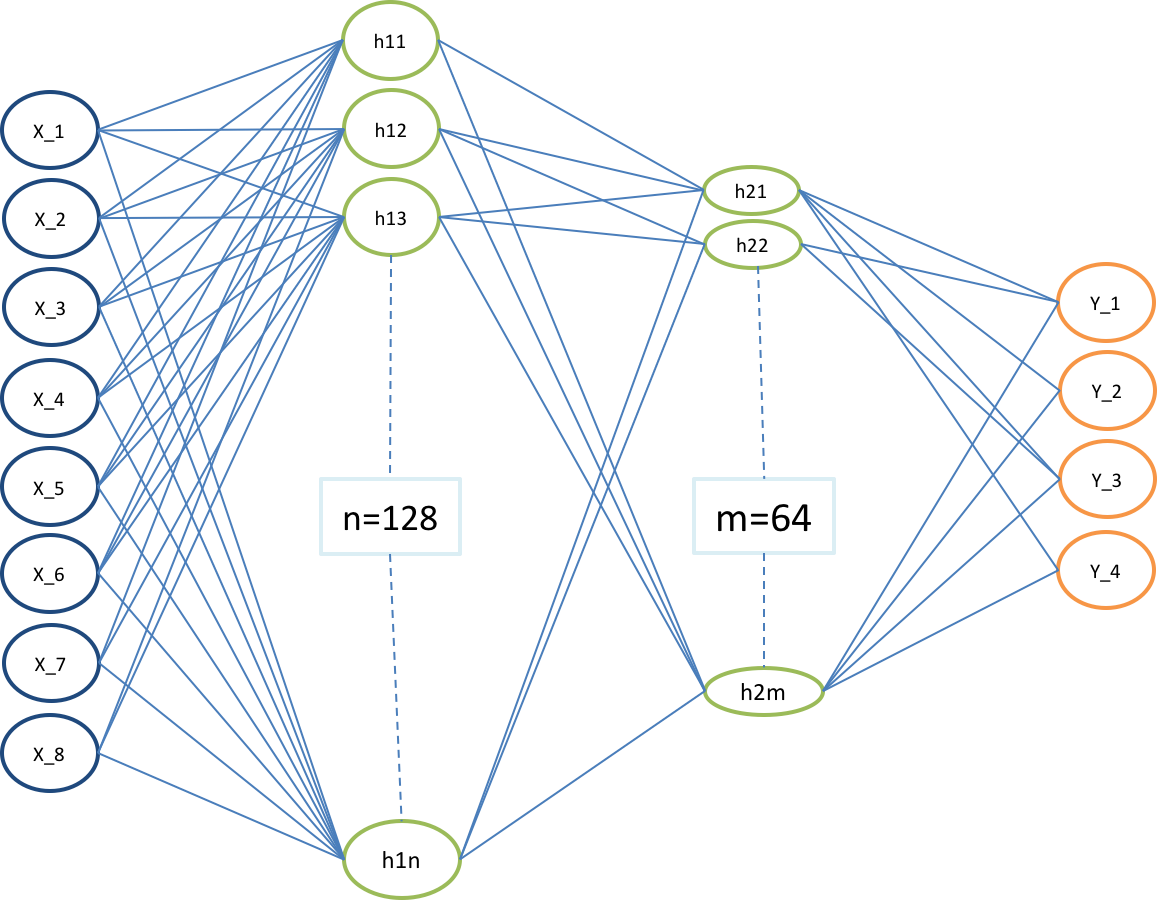
\includegraphics[scale=0.35,width=0.35\columnwidth]{figures/NN.png}%
\caption{ DQN with two layers used to model the agent }%
\label{fig:Visualization}%
\end{figure}
%\vfill}

To overcome this problem, researches proposed to use a separate target network for setting the targets. From here on whenever we refer to DQN we mean Full DQN.

\subsubsection{Double DQN}
One problem in the DQN algorithm is that the agent tends to overestimate the Q function value, due to the max in the formula used to set targets.
Because of the max in the formula, the action with the highest positive/negative error could be selected and this value might subsequently propagate further to other states. This leads to bias – value overestimation. This severe impact on stability of the learning algorithm.
\newline
In this new algorithm, two Q functions $Q_{1}$ and $Q_2$ – are independently learned. One function is then used to determine the maximizing action and second to estimate its value. Either $Q_1$ or $Q_2$ is updated randomly with a formula:
\begin{equation}
Q_1(s, a) \xrightarrow{} r + \gamma Q_2(s', argmax_a Q_1(s', a)) 
\end{equation}
or
\begin{equation}
Q_2(s, a) \xrightarrow{} r + \gamma Q_1(s', argmax_a Q_2(s', a)) 
\end{equation}
It was proven that by decoupling the maximizing action from its value in this way, one can indeed eliminate the maximization bias.
\newline
When thinking about implementation into the DQN algorithm, we can leverage the fact that we already have two different networks giving us two different estimates Q and $\tilde{Q}$ (target network). Although not really independent, it allows us to change our algorithm in a really simple way.
\newline
The original target formula would change to:
\begin{equation}
Q(s, a) \xrightarrow{} r + \gamma \tilde{Q}(s', argmax_a Q(s', a))
\end{equation}
We could observe that Double DQN was more stable than Full DQN.
 
\subsubsection{Dueling layer DQN}


In Dueling DQN, Q is computed with a different formula below with value function V and a state-dependent action advantage function A below:

\begin{equation}
Q(s,a) \rightarrow V(s) + A(s,a) -\frac{1}{A} \sum_{a'}^{} A(s,a )
\end{equation}

Instead of learning Q, we used two separate heads to compute V and A.Our experiments show the performance improvements. DQN updates the Q-value function of a state for a specific action only. Dueling DQN updates V which other Q(s, a’) updates can take advantage of also. So each Dueling DQN training iteration is thought to have a larger impact.
\\
The insight behind the dueling network architecture is that sometimes the exact choice of action does not matter so much, and so the state could be more explicitly modeled, independent of the action. There are two neural networks — one learns to provide an estimate of the value at every timestep, and the other calculates potential advantages of each action, and the two are combined for a single action-advantage Q function. We can achieve more robust estimates of state value by decoupling it from the necessity of being attached to specific actions.\citep{Dueling}
\newline
\begin{equation}
Q(s,a) \rightarrow A(s,a) + V(s)
\end{equation}
\newline 

\begin{figure}[!ht]
%\begin{figure}%
%\vspace*{\fill}
%\centering
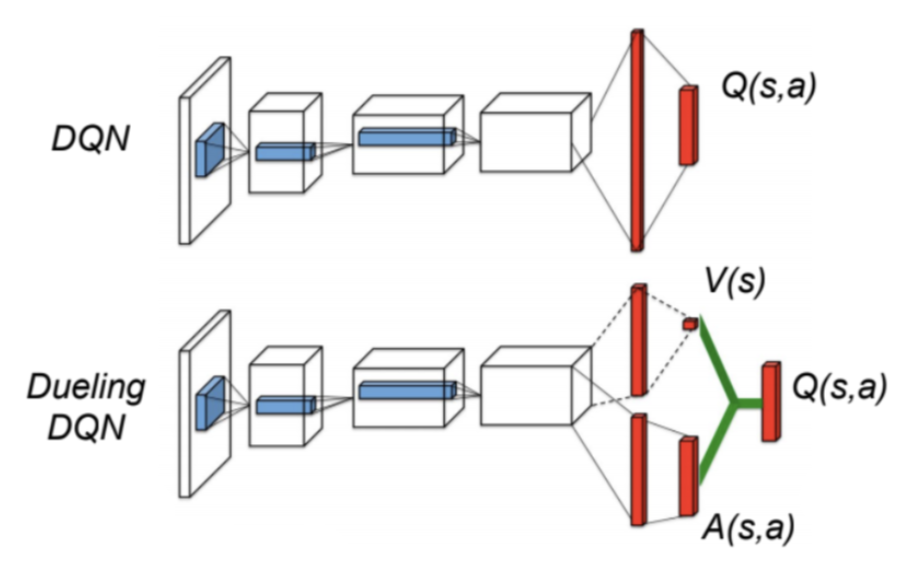
\includegraphics[scale=0.50,width=0.50\columnwidth]{figures/DuelingArch.png}%
\caption{ DQN and Dueling DQN Architeture\citep{Dueling_Diagram}}%
\label{fig:Dueling and DQN Architecture}%
\end{figure}

\subsection{Accuracy and Efficiency Trade-off}

For our solutions, accuracy can be considered as consistency in getting more than 200 scores over a period of episodes. And efficiency would be how sooner we can get such weights for which the agent scores more than 200 scores. \\

When we train for more number of episodes (low efficiency) we converge better and rewards are consistently better (more than 200), contributing to high accuracy(drop between consecutive episodes is lesser). But if we stop early(at 400 episodes) , we are highly efficient( but the accuracy is lower). It is evident from the smoothness in average rewards post 600 episodes (Tensorboard curve shown in Figure 6).


